\section{Popularity}
Using Google Trends we can analyse the popularity of search queries performed across Google. The results can be found in \autoref{fig:google-trends-result}.

According to Google the interest numbers represent the search interest relative to the highest point on the chart for the given region and time. A value of 100 is the peak popularity for the term. A value of 50 means that the term is half as popular. A score of 0 means that there was not enough data for this term.

Although these graphs give a certain representation they are far from ideal. They should be assessed in a critical fashion.

For instance Figma is considered the clear winner here. It is not accurate. Figma is also the name of a Japanese action figure line which increases the amount of queries . This can be seen in \autoref{app:google-trends-queries-figma} where one of the related searches is "edelgard figma" which is indeed an action figure. There are few other trivial keywords.

You may also have noticed Sketch is not included in the comparison. First and foremost because the word 'sketch' is a word with multiple meanings. It is also a drawing and a short humorous play. Google Trends is able to Sketch as a software tool, unfortunately, the other tools are not acknowledged, thus the data is not trust-worthy.

This makes the interest results inaccurate. Besides that the Google Trends website is limited to 5 search terms at once.

 Screen capture taking from \url{https://trends.google.com/trends/explore?q=Adobe\%20XD,InVision,Framer,Figma,Axure}.
\begin{figure}[H]
    \centering
    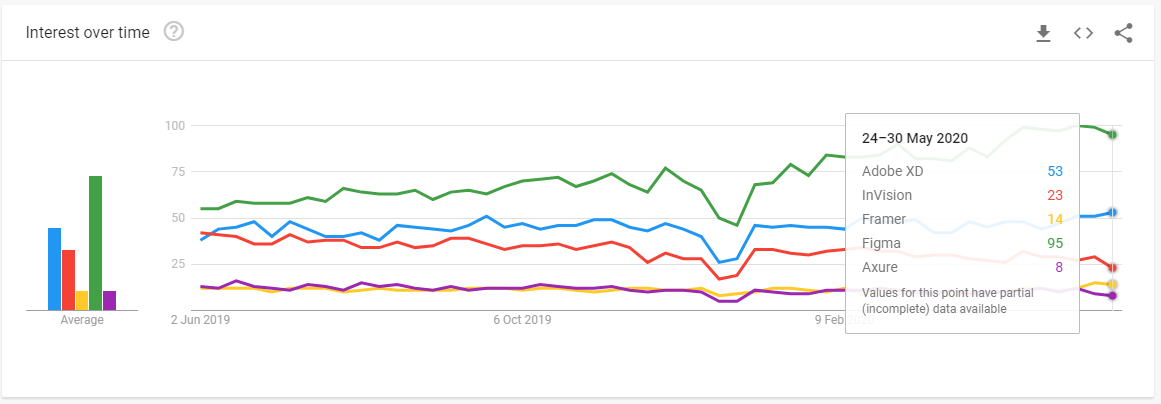
\includegraphics[scale=0.45]{figures/trends/google-trends.png}
    \caption{Google Trends interest results}
    \label{fig:google-trends-result}
\end{figure}
   
You can see detailed trend results of each tool individually in the screen captures in \autoref{app:google-trends}.
The results can also be found on the Google Trends website:  \url{https://trends.google.com/trends/explore?q=Adobe\%20XD,InVision,Framer,Figma,Axure}. Mind you, the results may be completely different at the time you open it, since it is real time data.


